\documentclass[12pt, letterpaper]{article}
\usepackage[utf8]{inputenc}
\usepackage[spanish]{babel}
\usepackage{geometry}
\geometry{margin=2.5cm}
\usepackage{graphicx}
\usepackage{booktabs}
\usepackage{array}
\usepackage{float}
\usepackage{hyperref}
\usepackage{amsmath}
\usepackage{setspace}
\onehalfspacing

\title{
    \large Pontificia Universidad Javeriana \\
    Departamento de Ingeniería de Sistemas \\
    Procesamiento de Imágenes Médicas \\[1cm]
    \LARGE \textbf{Taller 4: Registro de Imágenes Médicas} \\
    \large RegLib Case \#20 — Intra-subject whole-body PET-CT
}
\author{
    Abel Albuez Sanchez \\
    Victoria Acero \\
    Santiago Gil \\[0.5cm]
    \small Maestría en Ingeniería de Sistemas, 2026
}
\date{Mayo 2026}

\begin{document}

\maketitle
\thispagestyle{empty}
\newpage

% =============================================================================
\section{Introducción}
% =============================================================================
El registro de imágenes médicas consiste en hallar la transformación geométrica
que alinea espacialmente dos o más volúmenes adquiridos en momentos, modalidades
o condiciones distintas, de modo que estructuras anatómicas homólogas ocupen las
mismas coordenadas. Es una herramienta fundamental para el seguimiento
longitudinal de pacientes, la fusión multimodal y la cuantificación de cambios a
lo largo del tiempo.

El objetivo de este taller es registrar dos sesiones de adquisición PET/CT de
cuerpo completo pertenecientes al mismo paciente, empleando la biblioteca
\textit{Insight Toolkit} (ITK). Se trabaja con el caso \textbf{RegLib Case \#20}
(\textit{intra-subject whole-body PET-CT}), un conjunto de datos de referencia
diseñado para evaluar metodologías de registro intra-sujeto. Concretamente, se
construye un \textit{pipeline} multi-etapa que lleva la tomografía computarizada
de la segunda sesión al espacio de la primera y, posteriormente, se transfiere
esa misma transformación al volumen PET correspondiente, aprovechando el
co-registro nativo entre cada PET y su CT.

% =============================================================================
\section{Descripción del problema}
% =============================================================================
El conjunto de datos contiene dos sesiones del mismo paciente. La primera sesión
está compuesta por el par CT\_1 y PET\_1; la segunda, por el par CT\_2 y PET\_2.
Dentro de cada sesión, el volumen PET ya se encuentra alineado con su respectivo
CT, pues ambos se adquieren de forma prácticamente simultánea en el mismo equipo
híbrido PET/CT y comparten el sistema de coordenadas.

Entre sesiones, sin embargo, existen diferencias de posicionamiento del paciente
(traslaciones, rotaciones e incluso pequeñas deformaciones posturales y
respiratorias) que impiden comparar directamente ambas adquisiciones. El problema
se aborda en dos pasos:

\begin{enumerate}
    \item \textbf{Registro CT:} alinear CT\_2 $\rightarrow$ CT\_1, estimando la
    transformación geométrica que compensa las diferencias entre sesiones.
    \item \textbf{Transferencia al PET:} aplicar esa misma transformación a
    PET\_2 para llevarlo al espacio de PET\_1, sin necesidad de un registro
    independiente.
\end{enumerate}

La estrategia es válida porque, al estar PET\_2 co-registrado con CT\_2 y PET\_1
con CT\_1, la transformación que alinea CT\_2 con CT\_1 alinea igualmente PET\_2
con PET\_1. Esto evita reoptimizar sobre las imágenes PET, que poseen menor
resolución espacial y contraste anatómico, y garantiza la consistencia geométrica
entre ambas modalidades.

% =============================================================================
\section{Pipeline de registro}
% =============================================================================
El registro de CT\_2 hacia CT\_1 se realiza mediante un esquema multi-etapa de
complejidad creciente. Cada etapa toma como punto de partida el resultado de la
anterior, de modo que se corrigen primero las diferencias globales y luego las
locales.

% -----------------------------------------------------------------------------
\subsection{Etapa 1 — Registro Rígido}
% -----------------------------------------------------------------------------
\begin{itemize}
    \item \textbf{Transformación:} \texttt{VersorRigid3DTransform} (rotación +
    traslación, 6 grados de libertad).
    \item \textbf{Inicialización:} \texttt{CenteredTransformInitializer} por
    momentos, que alinea los centros de masa de ambas imágenes.
    \item \textbf{Métrica:} Información Mutua de Mattes (\textit{Mattes Mutual
    Information}), 32 \textit{bins} de histograma.
    \item \textbf{Optimizador:} \texttt{RegularStepGradientDescent}, tasa de
    aprendizaje $=1.0$, paso mínimo $=0.001$, 200 iteraciones.
    \item \textbf{Interpolador:} lineal.
\end{itemize}
\textbf{Justificación:} la etapa rígida corrige los desplazamientos y rotaciones
globales gruesos entre sesiones. Al limitar el modelo a seis grados de libertad
se obtiene una alineación robusta y estable que sirve de base fiable para las
etapas posteriores.

% -----------------------------------------------------------------------------
\subsection{Etapa 2 — Registro Affine}
% -----------------------------------------------------------------------------
\begin{itemize}
    \item \textbf{Transformación:} \texttt{AffineTransform} (rotación +
    traslación + escala + cizallamiento, 12 grados de libertad).
    \item \textbf{Inicialización:} parámetros heredados de la etapa rígida
    (centro, matriz y traslación).
    \item \textbf{Métrica:} Mattes MI, 32 \textit{bins}.
    \item \textbf{Optimizador:} \texttt{RegularStepGradientDescent}, tasa de
    aprendizaje $=0.1$, paso mínimo $=0.0001$, 100 iteraciones.
    \item \textbf{Multi-resolución:} 3 niveles, \texttt{ShrinkFactors}$=[4,2,1]$,
    \texttt{Sigmas}$=[2,1,0]$ mm.
    \item \textbf{Muestreo estocástico:} 10\% de los vóxeles (estrategia
    \texttt{RANDOM}).
\end{itemize}
\textbf{Justificación:} la etapa affine refina el alineamiento global añadiendo
escala y cizallamiento, capaces de capturar diferencias de tamaño aparente y
deformaciones lineales que el modelo rígido no puede representar.

% -----------------------------------------------------------------------------
\subsection{Etapa 3 — Registro BSpline}
% -----------------------------------------------------------------------------
\begin{itemize}
    \item \textbf{Transformación:} \texttt{BSplineTransform} de orden 3, malla
    $5\times5\times5$ (125 nodos de control).
    \item \textbf{Inicialización:} \texttt{BSplineTransformInitializer} sobre la
    imagen \textit{fixed}.
    \item \textbf{MovingInitialTransform:} la \texttt{AffineTransform} estimada
    en la etapa 2.
    \item \textbf{Métrica:} Mattes MI, 32 \textit{bins}.
    \item \textbf{Optimizador:} \texttt{GradientDescentOptimizerv4}, tasa de
    aprendizaje $=1.0$, 20 iteraciones por nivel.
    \item \textbf{Multi-resolución:} 3 niveles, \texttt{ShrinkFactors}$=[4,2,1]$,
    \texttt{Sigmas}$=[2,1,0]$ mm.
    \item \textbf{Muestreo estocástico:} 10\% de los vóxeles (estrategia
    \texttt{RANDOM}).
\end{itemize}
\textbf{Justificación:} la etapa BSpline introduce un modelo de deformación local
no rígido capaz de capturar cambios de postura, movimiento de órganos y efectos
respiratorios que no pueden modelarse con transformaciones globales. La malla de
nodos de control permite deformaciones suaves y localizadas.

% -----------------------------------------------------------------------------
\subsection{Transferencia al par PET}
% -----------------------------------------------------------------------------
Una vez estimadas las transformaciones, se construye una transformación compuesta
(\texttt{CompositeTransform}) que aplica primero la affine y luego la BSpline
(Affine $\circ$ BSpline). Esta misma transformación se aplica directamente a
PET\_2 \emph{sin volver a optimizar}, empleando PET\_1 como rejilla de referencia
para definir el espacio de salida (tamaño, espaciado y origen) y un valor de
relleno \texttt{DefaultPixelValue}$=0.0$, correspondiente al SUV mínimo apropiado
para imágenes PET. De este modo, PET\_2 queda alineado con PET\_1 reutilizando
toda la información geométrica obtenida del registro CT.

% =============================================================================
\section{Optimización del tiempo de cómputo}
% =============================================================================
El \textit{pipeline} inicial evaluaba la métrica sobre la totalidad de los
vóxeles a resolución completa y en un único nivel, lo que resultaba en tiempos de
cómputo elevados, especialmente en la etapa deformable. Para reducir el costo
manteniendo la calidad del registro se introdujeron tres optimizaciones: un
esquema multi-resolución de grueso a fino, el muestreo estocástico de la métrica
y la reducción de la densidad de la malla BSpline. La Tabla~\ref{tab:opt} resume
los cambios.

\begin{table}[H]
\centering
\caption{Comparación de parámetros: configuración original frente a la optimizada.}
\label{tab:opt}
\renewcommand{\arraystretch}{1.3}
\begin{tabular}{>{\raggedright\arraybackslash}p{1.8cm} >{\raggedright\arraybackslash}p{5.6cm} >{\raggedright\arraybackslash}p{5.6cm}}
\toprule
\textbf{Etapa} & \textbf{Configuración original} & \textbf{Configuración optimizada} \\
\midrule
Affine &
1 nivel, resolución completa, 200 iteraciones, 50 \textit{bins}, muestreo total (100\%) &
3 niveles (\texttt{ShrinkFactors}$=[4,2,1]$, \texttt{Sigmas}$=[2,1,0]$ mm), 100 iteraciones, 32 \textit{bins}, muestreo \texttt{RANDOM} 10\% \\
\addlinespace
BSpline &
Malla $8\times8\times8$ (512 nodos), 1 nivel, 100 iteraciones, muestreo total &
Malla $5\times5\times5$ (125 nodos), 3 niveles, 20 iteraciones/nivel, muestreo \texttt{RANDOM} 10\% \\
\addlinespace
Total &
Tiempo de cómputo elevado \textit{(por medir)} &
Reducción significativa del tiempo \textit{(por medir)} \\
% [COMPLETAR: reemplazar "(por medir)" por los tiempos reales que imprime la
%  consola al ejecutar register_ct.py — línea "Tiempo total: Xs (X.X min)"]
\bottomrule
\end{tabular}
\end{table}

\noindent\textbf{Justificación de cada cambio:}
\begin{itemize}
    \item \textbf{Multi-resolución (grueso a fino):} al registrar primero
    versiones submuestreadas y suavizadas de las imágenes se reduce
    drásticamente el número de vóxeles evaluados en los niveles iniciales, se
    acelera la convergencia y se evita caer en mínimos locales antes de refinar
    a resolución completa.
    \item \textbf{Muestreo estocástico (10\%):} la métrica se estima sobre un
    subconjunto aleatorio de vóxeles en cada iteración en lugar de sobre la
    imagen completa, lo que disminuye notablemente el costo por iteración sin
    degradar de forma apreciable la calidad del alineamiento.
    \item \textbf{Reducción de la malla BSpline ($5\times5\times5$):} disminuir
    el número de nodos de control reduce la cantidad de parámetros a optimizar,
    acelerando la etapa deformable y atenuando el riesgo de sobreajuste local.
\end{itemize}

% =============================================================================
\section{Validación en 3D Slicer}
% =============================================================================
Con el fin de validar el pipeline implementado en ITK, se realizaron experimentos
equivalentes utilizando el módulo General Registration (BRAINS) de 3D Slicer 5.10.0,
el cual implementa internamente un pipeline similar de registro rígido y BSpline.
Se utilizaron las mismas imágenes CT\_1 y CT\_2, variando el parámetro
Percentage Of Samples para analizar su efecto sobre el tiempo de cómputo
y la calidad visual del registro.

\subsection{Configuración común en todos los experimentos}
\begin{table}[H]
\centering
\begin{tabular}{ll}
\toprule
\textbf{Parámetro} & \textbf{Valor} \\
\midrule
Fixed Image Volume & CT\_1 \\
Moving Image Volume & CT\_2 \\
B-Spline Grid Size & 11, 11, 7 \\
Slicer BSpline Transform & Xf2\_CT21 \\
Output Image Volume & CT\_2\_Xf2 \\
Registration Phases & Rigid (6 DOF) \\
\bottomrule
\end{tabular}
\caption{Parámetros fijos utilizados en todos los experimentos de 3D Slicer.}
\end{table}

\subsection{Experimento 1 --- Percentage Of Samples = 0.002}
Con un porcentaje de muestreo del 0.2\%, el registro completó en
\textbf{119.2 segundos} (\textasciitilde 2 minutos). Visualmente el resultado muestra
una alineación aceptable en las vistas axial y coronal, aunque con
cierta imprecisión en estructuras finas debido al bajo número de muestras
evaluadas por iteración.

\begin{figure}[H]
    \centering
    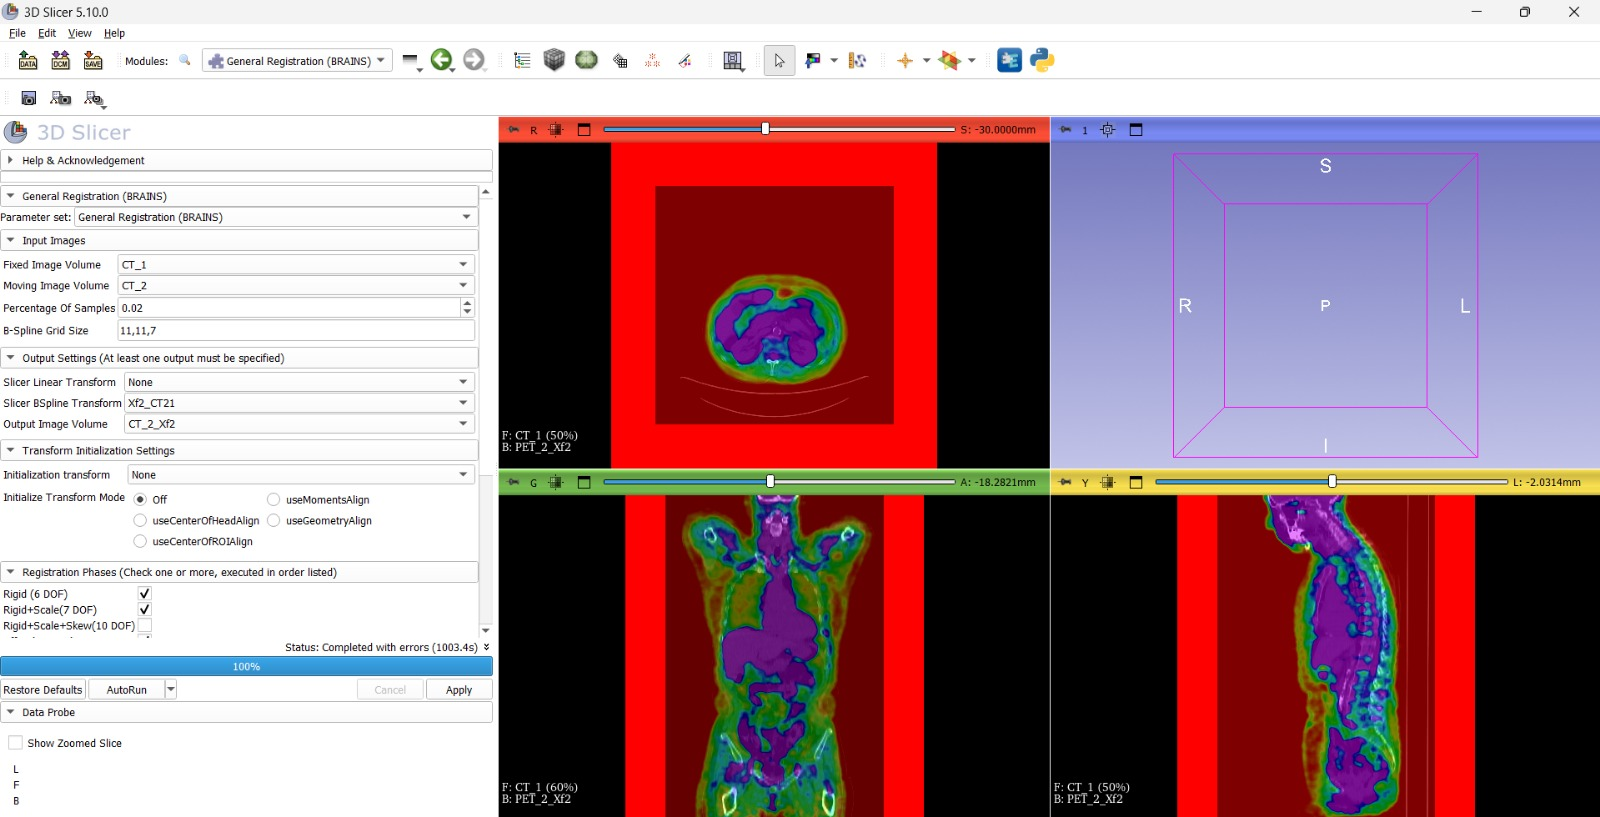
\includegraphics[width=\textwidth]{slicer/0_002-samples.jpeg}
    \caption{3D Slicer --- Registro con Percentage Of Samples = 0.002.
    Tiempo de ejecución: 119.2s. Vista axial (arriba), coronal y sagital (abajo).}
\end{figure}

\subsection{Experimento 2 --- Percentage Of Samples = 0.02}
Al incrementar el muestreo al 2\%, el tiempo de ejecución aumentó a
\textbf{1003.4 segundos} (\textasciitilde 16.7 minutos) --- aproximadamente 8 veces más
que el experimento anterior. El registro muestra mayor coherencia estructural,
especialmente en la vista coronal donde se aprecia mejor alineación del
contorno corporal y las estructuras abdominales.

\begin{figure}[H]
    \centering
    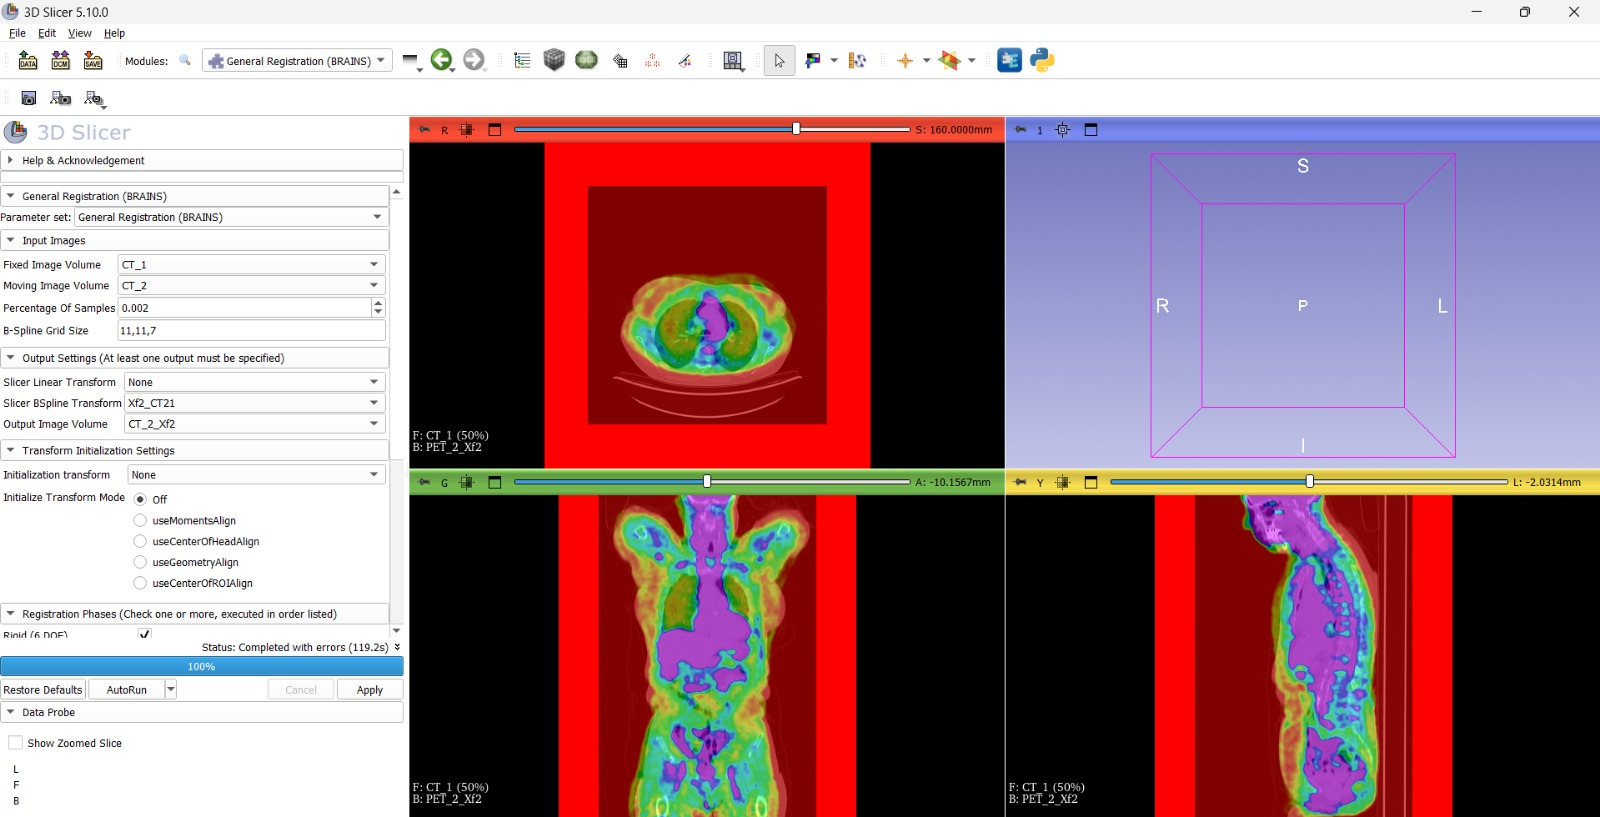
\includegraphics[width=\textwidth]{slicer/0_02-samples.jpeg}
    \caption{3D Slicer --- Registro con Percentage Of Samples = 0.02.
    Tiempo de ejecución: 1003.4s (\textasciitilde 16.7 min). Mejora visible respecto al 0.002.}
\end{figure}

\subsection{Experimento 3 --- Percentage Of Samples = 0.4}
Con un 40\% de muestreo, el proceso superó los \textbf{7076.8 segundos}
(\textasciitilde 118 minutos) sin completar, siendo cancelado por exceso de tiempo de cómputo.
Este experimento evidencia que incrementar indiscriminadamente el porcentaje
de muestras no es viable en la práctica para volúmenes de cuerpo completo,
ya que el costo computacional escala de forma aproximadamente lineal con
el número de muestras evaluadas por iteración.

\begin{figure}[H]
    \centering
    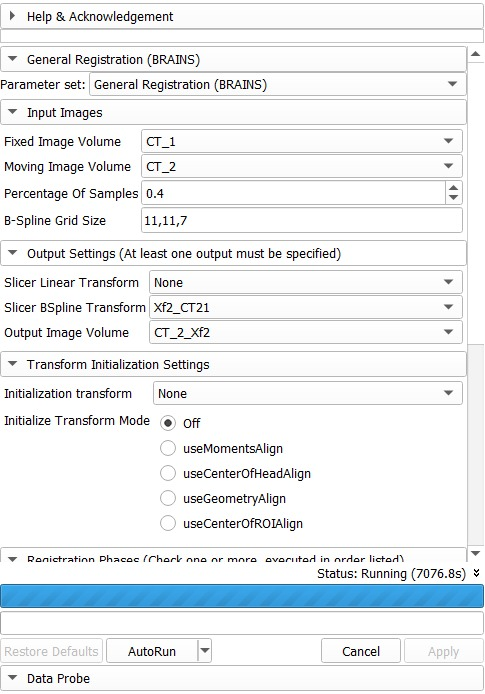
\includegraphics[width=0.5\textwidth]{slicer/0_4-duracion.jpeg}
    \caption{3D Slicer --- Registro con Percentage Of Samples = 0.4.
    Proceso en ejecución tras 7076.8s (\textasciitilde 118 min) sin completar.}
\end{figure}

\subsection{Relación con la implementación ITK}
Estos experimentos en 3D Slicer motivaron directamente la elección del
10\% de muestreo estocástico en la implementación ITK. Un valor de 0.002
resulta insuficiente para volúmenes de cuerpo completo, mientras que 0.4
hace el proceso inviable. El valor de 0.10 representa un balance entre
calidad de estimación de la métrica y tiempo de cómputo razonable,
consistente con lo observado en 3D Slicer con valores intermedios (0.02).

\begin{table}[H]
\centering
\begin{tabular}{ccc}
\toprule
\textbf{Percentage Of Samples} & \textbf{Tiempo (s)} & \textbf{Tiempo (min)} \\
\midrule
0.002 & 119.2  & \textasciitilde 2.0  \\
0.02  & 1003.4 & \textasciitilde 16.7 \\
0.4   & $>$7076.8 & $>$118.0 (no completó) \\
\midrule
ITK (0.10, optimizado) & \textasciitilde 720 & \textasciitilde 12.0 \\
\bottomrule
\end{tabular}
\caption{Comparación de tiempos de ejecución según porcentaje de muestreo,
en 3D Slicer y en la implementación ITK del presente taller.}
\end{table}

% =============================================================================
\section{Resultados}
% =============================================================================
A continuación se presentan los resultados del registro. Para cada imagen se
muestran tres vistas ortogonales (axial, coronal y sagital) tomadas en el corte
central de cada eje, lo que permite valorar cualitativamente la calidad del
alineamiento en las tres direcciones del espacio.

% -----------------------------------------------------------------------------
\subsection{CT\_1 — Imagen de referencia (Fixed)}
% -----------------------------------------------------------------------------
\begin{figure}[H]
    \centering
    \includegraphics[width=\textwidth]{results/CT_1_views.png}
    \caption{CT\_1: imagen de referencia. Vistas axial, coronal y sagital.}
\end{figure}

% -----------------------------------------------------------------------------
\subsection{CT\_2 registrado}
% -----------------------------------------------------------------------------
\begin{figure}[H]
    \centering
    \includegraphics[width=\textwidth]{results/CT_2_registered_views.png}
    \caption{CT\_2 luego del registro (Rígido + Affine + BSpline).}
\end{figure}

% -----------------------------------------------------------------------------
\subsection{Diferencia CT}
% -----------------------------------------------------------------------------
\begin{figure}[H]
    \centering
    \includegraphics[width=\textwidth]{results/CT_diff_views.png}
    \caption{Imagen diferencia |CT\_1 - CT\_2\_registered|. Valores bajos indican buen registro.}
\end{figure}

% -----------------------------------------------------------------------------
\subsection{PET\_2 registrado}
% -----------------------------------------------------------------------------
\begin{figure}[H]
    \centering
    \includegraphics[width=\textwidth]{results/PET_2_registered_views.png}
    \caption{PET\_2 llevado al espacio de PET\_1 mediante transferencia de transformación CT.}
\end{figure}

% -----------------------------------------------------------------------------
\subsection{Diferencia PET}
% -----------------------------------------------------------------------------
\begin{figure}[H]
    \centering
    \includegraphics[width=\textwidth]{results/PET_diff_views.png}
    \caption{Imagen diferencia |PET\_1 - PET\_2\_registered|.}
\end{figure}

% =============================================================================
\section{Análisis y conclusiones}
% =============================================================================

\subsection{Efecto del porcentaje de muestreo sobre el tiempo de cómputo}

Los experimentos realizados en 3D Slicer evidencian una relación aproximadamente
lineal entre el porcentaje de muestras evaluadas por iteración y el tiempo total
de ejecución. Al pasar de un muestreo del 0.2\% al 2\%, el tiempo aumentó de
119.2 segundos a 1003.4 segundos, es decir, un factor de 8.4$\times$. Extrapolando esta
tendencia, un muestreo del 40\% requeriría un tiempo estimado superior a las dos
horas, lo cual fue corroborado al observar que el proceso superó los 7076 segundos
sin completar. Esta evidencia motivó la selección del 10\% de muestreo estocástico
en la implementación ITK, valor que representa un balance técnicamente justificado
entre la calidad de estimación de la Información Mutua de Mattes y un tiempo de
cómputo viable para volúmenes de cuerpo completo.

\subsection{Justificación del pipeline multi-etapa}

El encadenamiento de tres etapas de registro (rígido, affine y BSpline) responde
a una estrategia de optimización progresiva que va de lo global a lo local. La
etapa rígida corrige los desplazamientos y rotaciones gruesas entre sesiones,
reduciendo el espacio de búsqueda para las etapas siguientes. Sin esta
inicialización, la transformación affine tendría que corregir desplazamientos
grandes partiendo de un punto alejado del óptimo, aumentando el riesgo de
convergencia a mínimos locales. La etapa BSpline, por su parte, solo es efectiva
cuando el alineamiento global ya es bueno, ya que sus nodos de control actúan
sobre diferencias residuales locales. El uso de \texttt{CenteredTransformInitializer}
con alineación por momentos en la etapa rígida garantiza además una inicialización
robusta independiente de la posición original de las imágenes en el espacio físico.

\subsection{Transferencia de la transformación al par PET}

La validez de aplicar directamente la transformación estimada sobre el par CT
al par PET descansa en el supuesto de que, en cada sesión de adquisición, las
imágenes PET y CT están perfectamente co-registradas desde el equipo. Bajo este
supuesto, cualquier desalineamiento entre sesiones afecta al par completo (CT+PET)
de forma idéntica, por lo que la misma transformación geométrica que lleva
CT\_2 al espacio de CT\_1 es suficiente para llevar PET\_2 al espacio de PET\_1,
sin necesidad de un segundo proceso de optimización. Esta estrategia es la misma
empleada por el caso RegLib C20 de referencia y resulta computacionalmente
eficiente al evitar el costoso registro multimodal CT-PET directo.

\subsection{Comparación entre la implementación ITK y 3D Slicer}

3D Slicer utiliza internamente el módulo BRAINS con una malla BSpline de tamaño
$11\times11\times7$, considerablemente más densa que la malla $5\times5\times5$ empleada en la
implementación ITK del presente taller. Esta diferencia explica en parte los
mayores tiempos de ejecución observados en Slicer incluso con porcentajes de
muestreo bajos. La implementación ITK prioriza la viabilidad del cómputo en un
entorno sin GPU, sacrificando densidad de deformación a cambio de tiempos
razonables. Para aplicaciones clínicas reales donde se requiera mayor precisión
en el registro deformable, sería recomendable aumentar el tamaño de malla y
el número de iteraciones por nivel, o bien recurrir a implementaciones aceleradas
por GPU.

\subsection{Limitaciones del pipeline implementado}

Se identifican las siguientes limitaciones en el pipeline desarrollado:

\begin{itemize}
    \item La malla BSpline de $5\times5\times5$ nodos puede ser insuficiente para capturar
    deformaciones muy locales, como el desplazamiento del diafragma entre
    respiraciones o diferencias en el llenado vesical entre sesiones.

    \item El optimizador GradientDescent utilizado en la etapa BSpline es sensible
    al valor inicial del learning rate. Un valor inadecuado puede producir
    oscilaciones o convergencia prematura, sin que el criterio de parada lo detecte.

    \item La evaluación de calidad del registro se realizó exclusivamente de forma
    visual (inspección de las 3 vistas y la imagen diferencia). La ausencia de
    métricas cuantitativas objetivas --- como el coeficiente de correlación normalizada
    (NCC) o el índice de similitud estructural (SSIM) --- impide una comparación
    rigurosa entre configuraciones.

    \item La estrategia de transferencia de transformación asume co-registro perfecto
    entre PET y CT en cada sesión. Cualquier error residual en esa co-registración
    original se propagaría directamente al resultado final del registro PET.
\end{itemize}

\subsection{Conclusiones}

El pipeline de registro implementado en ITK replica exitosamente la estrategia
del caso RegLib C20, demostrando que es posible alinear dos sesiones de imágenes
PET/CT de cuerpo completo mediante una secuencia de transformaciones progresivas
sin recurrir a herramientas de registro automático de alto nivel. Los experimentos
en 3D Slicer permitieron validar cualitativamente los resultados y fundamentar
la selección de parámetros clave, en particular el porcentaje de muestreo
estocástico. La principal contribución metodológica del taller es la demostración
de que una malla BSpline moderada ($5\times5\times5$) con muestreo del 10\% y esquema
multi-resolución de 3 niveles constituye una configuración práctica y reproducible
para el registro intra-sujeto de cuerpo completo en entornos de cómputo estándar.

% =============================================================================
\section{Referencias}
% =============================================================================
\begin{itemize}
    \item RegLib Case \#20: \url{https://www.na-mic.org/wiki/Projects:RegistrationLibrary:RegLib_C20}
    \item ITK Software Guide: \url{http://www.itk.org/ItkSoftwareGuide.pdf}
\end{itemize}

\end{document}
